\documentclass[10pt,a4paper]{article}

\usepackage[margin=1.5cm]{geometry}
\usepackage[UKenglish]{babel}
\usepackage{enumitem}
\usepackage{fancyhdr}
\usepackage{graphicx}

\pagestyle{fancy}
\lhead{T Davies, A Fahie, A Fairbairn, A Free, J Mansfield, R Tucker, M Walker}
\chead{}
\rhead{GPIG-C}
\cfoot{}

\setlist{nolistsep} % Reduces lots of white space around lists

\renewcommand{\headrulewidth}{0.4pt} % Add rules below header
\renewcommand{\footrulewidth}{0.4pt}

\begin{document}

\title{\vspace{-1cm}GPIG-C Initial Report}
\author{}
\date{\vspace{-1cm} Friday, 25th October}
\maketitle
\thispagestyle{fancy} % Make sure header and footer appear on the front page

\section{Introduction}
\subsection{Single Statement of Need}
This project aims to deliver a tailorable Health and Usage Monitoring System (HUMS), tailorable to multiple target domains. The target for the system is any consumer needing to collect, store, analyse and report data from one or more data input clients.
\subsection{Intended Audience of this Document}
The intended audience of this document are both the developers and the customer. The document is structured in a manner which will interest all concerned parties. Requirements will follow the introduction, followed by use cases, a review of possible solutions and a risk register.

\section{Use cases}
\noindent \textbf{ID:} UC1\\
\textbf{Name:} Monitoring a system.\\
\textbf{Context:} The organisation has developed a system, for which they require health and usage monitoring.\\
\textbf{Primary Actor:} The organisation's technical representative.\\
\textbf{Secondary Actors:} The health and usage monitoring system, the organisation's system.\\
\textbf{Precondition:}  The organisation has a system that requires monitoring. The organisation's system and environment must conform to the constraint requirements detailed in this document. The end user has access to the facilities required to install the HUMS. The end user has basic technical computing knowledge.\\
\textbf{Trigger:} The end user sets up an account and attempts to integrate their system.\\
\textbf{Main Success Scenario:} The end user successfully manages to integrate their system with the HUMS.\\
\textbf{Main Success Postcondition:} The HUMS is successfully integrated with the user's system, allowing data to be passed through the input and output interfaces.\\
\textbf{Exception Scenarios:}
\begin{itemize}
\item The end user fails to integrate their system with the HUMS because their system does not conform to the data input interface.
\item The end user fails to integrate their system with the HUMS because their system does not conform to the output interface.
\item The end user chooses to abort the process.
\end{itemize}
\textbf{Exception Postcondition:} If the end user's system could not be integrated with the HUMS, the user is provided with diagnostic information and technical support needed to solve any problems. If the end user chose to quit the process, they are presented with access to technical support.\\\\

\noindent \textbf{ID:} UC2\\
\textbf{Name:} Analysing collected data.\\
\textbf{Context:} The organisation wishes to define how their data should be analysed.\\
\textbf{Primary Actor:} The end user.\\
\textbf{Secondary Actors:} The HUMS.\\
\textbf{Precondition:}
\begin{itemize}
\item The user has set up an account.
\item The organisation's sensor system and the HUMS have been successfully integrated.
\end{itemize}
\textbf{Trigger:} The user decides how they want to analyse their data abstractly.\\
\textbf{Main Success Scenario:}
\begin{itemize}
\item The user creates a concrete implementation of their abstract analysis system and interfaces it with the HUMS, allowing them to analyse data as per their definition.
\item We implement an analysis system on the user's behalf. The HUMS then analyses data as as defined by the user.
\end{itemize}
\textbf{Main Success Postcondition:} User can analyse data stored in the HUMS.\\
\textbf{Exception Scenarios:} User's analysis system does not conform to the analysis interface.\\
\textbf{Exception Postcondition:} HUMS can still collect and store data.\\\\

\noindent \textbf{ID:} UC3\\
\textbf{Name:} Reporting and notifications\\
\textbf{Context:} The organisation's sensor system, analysis system and the HUMS have been successfully integrated, and they now wish to define how users should be notified of events or receive reports.\\
\textbf{Primary Actor:} End user\\
\textbf{Secondary Actors:} The HUMS.\\
\textbf{Precondition:}
\begin{itemize}
\item The user has set up an account
\item The organisation's sensor system, analysis system and the HUMS have been successfully integrated.
\end{itemize}
\textbf{Trigger:} The user decides on the format and communication method used to keep them informed of the state of the system.\\
\textbf{Main Success Scenario:}
\begin{itemize}
\item The user implements a notification and reporting system with correctly integrates with the HUMS to keep end users informed.
\item We implement a notification and reporting system on behalf of the customer, allowing them to receive updates about the state of the system they are monitoring.
\end{itemize}
\textbf{Main Success Postcondition:}
\begin{itemize}
\item The user is notified when the analysis system fires an event
\item The user can request reports
\end{itemize}
\textbf{Exception Scenarios:} User's notification and reporting system implementation does not conform to the notification and reporting interface and so cannot function correctly.\\
\textbf{Exception Postcondition:} HUMS can still collect, store and analyse data.

\section{Requirements}
For this project, requirements have been divided into three categories, functional, non-functional and constraint. The requirements have been engineered such that each falls into one of those three categories, this prevents them from becoming too complex. Each requirement has been structured as simply and concisely as possible and been worded in such a way as to avoid ambiguity. The requirements represent the problem to be solved and serve as a contract between us, as the development team, and the customer. All requirements have therefore been checked with the customer to ensure the system described is the system they envisioned.\\
The functional requirements detail what inputs, behaviour and outputs the system must provide. The non-functional requirements specify the qualities of the system as opposed to its behaviour. Constraint requirements are those that apply to the entire system, including any constraints on the environment the system can be used in and any timing constraints. In order to ensure all requirements are verifiable, appropriate testing procedures have been included.

\subsection{Functional Requirements}
\subsubsection{Sensing Data}
\begin{table}[H]
\vspace{-0.5cm}
    \begin{tabular}{| p{1.1cm} | p{6cm} | p{9cm} | }
    	\hline
    	\cellcolor{titleColor}\textbf{ID}   & \cellcolor{titleColor}\textbf{Description}                                                              & \cellcolor{titleColor}\textbf{Verification}                                                                                                                                                                                                                                     \\ \hline
    	\textbf{FR.1} & Data input clients shall be able to push correctly structured data to the system. & Unit Testing 
	\begin{itemize} 
	\item Attempt to send correctly structured data to the system. Assert the data is correctly received.
	 \item Attempt to send incorrectly structured data to the system. Assert the data failed structure validation.
	 \end{itemize} \\ \hline
    	\textbf{FR.2} & The system shall allocate a timestamp to new data.                                & Unit Testing\begin{itemize} \item Assert data is timestamped.\item Assert there is a ��happens before�� relation between any pair of timestamps, such that timestamps reflect the order in which data arrives.\end{itemize}\\ \hline
	\end{tabular}
\end{table}
\subsubsection{Storing Data}
\begin{table}[H]
\vspace{-0.5cm}
    \begin{tabular}{| p{1.1cm} | p{6cm} | p{9cm}| }
        \hline
        \cellcolor{titleColor}\textbf{ID}    & \cellcolor{titleColor}\textbf{Description}                                                                                                                           & \cellcolor{titleColor}\textbf{Verification}                                                                                                                                                                                                                                                                    
        \\ \hline
        \textbf{FR.3}  & The system shall store correctly structured data.                                                                                              & Unit Testing\begin{itemize} \item Attempt to store correctly structured data in the system. Assert that the data can be retrieved.\item Attempt to store incorrectly structured data in the system. Assert that the data is rejected.\end{itemize}                                \\ \hline
        \textbf{FR.4}  & The system shall allow the consumer to define a low storage threshold.                                                                         & Black Box Testing\begin{itemize} \item Attempt to set a low storage threshold. Assert attempt is successful.\end{itemize}                                                                                                                                                           \\ \hline
        \textbf{FR.5}  & The system shall send a notification when the consumers defined low storage threshold is reached.                                              & Unit Testing\begin{itemize} \item Simulate reaching the low storage threshold. Assert that the method invoking a notification is called.\end{itemize}                                                                                                                               \\ \hline
        \textbf{FR.6}  & The system shall allow the consumer to set an expiry time on data.                                                                             & Grey Box Testing\begin{itemize} \item Attempt to set an expiry time on data. Add the data to the system. Assert the data has been stored with the expiry time.\end{itemize}                                                                                                         \\ \hline
        \textbf{FR.7}  & The system will delete data when its expiry time is reached.                                                                                   & Integration Testing\begin{itemize} \item Assert no stored data is older than its defined expiry time.\end{itemize}                                                                                                                                                                  \\ \hline
        \textbf{FR.8}  & The system must store no more data records than the consumers defined storage quota.                                                           & Integration Testing\begin{itemize} \item Assert the maximum number of data records held by the consumer is less than or equal to their defined quota.\end{itemize}                                                                                                                  \\ \hline
        \textbf{FR.9}  & The system shall allow the user to define that, upon reaching their defined data storage quota, new data is no longer added.                   & Unit Testing\begin{itemize} \item Simulate reaching the an arbitrary storage quota. Attempt to send more data to the system. Assert the send failed due to insufficient storage.\end{itemize}                                                                                       \\ \hline
    	\textbf{FR.10} & The system shall allow the user to define that, upon reaching their defined data storage limit, old data is deleted to make room for new data. & Unit Testing\begin{itemize} \item Simulate reaching the an arbitrary storage quota. Attempt to send more data to the system. Assert the send succeeded and the new data has been added to storage. Assert that the previous oldest record in storage has been deleted.\end{itemize} \\ \hline
	\end{tabular}
\end{table}
\subsubsection{Analysing Data}
\begin{table}[H]
\vspace{-0.5cm}
    \begin{tabular}{| p{1.1cm} | p{6cm} | p{9cm} |}
        \hline
        \cellcolor{titleColor}\textbf{ID}    & \cellcolor{titleColor}\textbf{Description}                                                                                      & \cellcolor{titleColor}\textbf{Verification}                                                                                                                                     \\ \hline
        \textbf{FR.11} & The system shall allow the consumer to specify what patterns of data will produce events.                 & Black Box Testing\begin{itemize} \item Assert that a specification of a valid pattern within a valid set of data succeeds.\end{itemize}              \\ \hline
        \textbf{FR.12} & Events shall be triggered in response to new data that matches a pattern that the consumer has specified. & Unit Testing\begin{itemize} \item Send the system a pattern of data which is known to constitute an event. Assert an event is produced.\end{itemize} \\ \hline
    \end{tabular}
\end{table}
\subsubsection{Reporting Events}
\begin{table}
    \begin{tabular}{| p{1.5cm}| p{6cm}| p{9cm}|}
        \hline
        \cellcolor{titleColor}\textbf{ID}    & \cellcolor{titleColor}\textbf{Description}                                                                                                                                              & \cellcolor{titleColor}\textbf{Verification}                                                                                                                                                                                                                                                                                                                                      \\ \hline
        \textbf{FR.13} & The system shall dispatch a notification to the data output client after an event has occurred.                                                                  & Unit Testing\begin{itemize}\item Simulate an event occurring. Assert that the method producing a notification is invoked.\end{itemize}                                                                                                                                                                                                               \\ \hline
        \textbf{FR.14} & The consumer shall be able to assign types to events.                                                                                                            & Black Box Testing\begin{itemize}\item Attempt to assign a valid type to a valid event. Assert the attempt is successful.\end{itemize}                                                                                                                                                                                                                \\ \hline
        \textbf{FR.15} & The consumer shall be able to assign a cool down period for each type of event.                                                                                  & Grey Box Testing\begin{itemize}\item Simulate the customer setting a cool down period. Assert the attempt is successful.\end{itemize}                                                                                                                                                                                                                \\ \hline
        \textbf{FR.16} & After the sending of a notification for an event of a particular type, no more notifications for an event of that type will be sent during the cool down period. & Black Box Testing\begin{itemize}\item Simulate the customer setting a cool down period and then multiple events of the same type being triggered. Assert only one notification during each cool down period is sent.\end{itemize}                                                                                                                    \\ \hline
        \textbf{FR.17} & The system must allow data output clients to pull reports from the system.                                                                                       & Unit Testing\begin{itemize}\item Attempt to pull a data report from the system. Assert attempt is successful. Assert received data is correct.\end{itemize}                                                                                                                                                                                          \\ \hline
        \textbf{FR.18} & The system shall allow the consumer to set which data output clients can pull reports.                                                                           & Unit Testing\begin{itemize}\item Attempt to set which output clients can pull reports.\item Attempt to send a report to an output client who is allowed to receive them and verify that it succeeds.\item Attempt to send a report to an output client who is not allowed to receive them and verify that it fails.\end{itemize}                 \\ \hline
    	\textbf{FR.19} & The system shall allow the consumer to set which output clients can be sent notifications.                                                                       & Unit Testing\begin{itemize}\item Attempt to set which output clients can be sent notifications.\item Attempt to send a notification to an output client who is allowed to receive them and verify that it succeeds.\item Attempt to send a notification to and output client who is not allowed to receive them and verify that it fails.\end{itemize} \\ \hline
	\end{tabular}
\end{table}


\subsection{Non-functional requirements}

\subsubsection{Maintainability}
\begin{table}[h!]
\vspace{-0.5cm}
    \begin{tabular}{|p{1.5cm}|p{6.0cm}|p{9.0cm}|}
    \hline
    \cellcolor{titleColor}\textbf{ID} & \cellcolor{titleColor}\textbf{Description} & \cellcolor{titleColor}\textbf{Verification} \\ \hline
    \textbf{NFR.1} & The system shall be able to receive hardware changes without loss of previously stored data. & Recovery Testing\begin{itemize}\item Take a snapshot of a live system. Change a piece of hardware on the system and then check that, after the change, the data is still consistent with the snapshot.\end{itemize} \\ \hline
    \end{tabular}
\end{table}

\subsubsection{Accessibility}
\begin{table}[h!]
\vspace{-0.5cm}
    \begin{tabular}{|p{1.5cm}|p{6.0cm}|p{9.0cm}|}
    \hline
    \cellcolor{titleColor}\textbf{ID} & \cellcolor{titleColor}\textbf{Description} & \cellcolor{titleColor}\textbf{Verification} \\ \hline
    \textbf{NFR.2} & Users shall be provided with documentation detailing how to use the system. & Acceptance Testing\begin{itemize}\item We will require a receipt verifying the availability and standard of the documentation when allowing the user access to the system documentation.\end{itemize} \\ \hline
    \textbf{NFR.3} & The system, when running externally on servers, must be accessible to end users who are in multiple geographic locations. & Black Box Testing\begin{itemize}\item Assert the networked system can be accessed from multiple geographic locations.\end{itemize} \\ \hline
    \end{tabular}
\end{table}

\subsubsection{Security}
\begin{table}[h!]
\vspace{-0.5cm}
    \begin{tabular}{|p{1.5cm}|p{6.0cm}|p{9.0cm}|}
    \hline
    \cellcolor{titleColor}\textbf{ID} & \cellcolor{titleColor}\textbf{Description} & \cellcolor{titleColor}\textbf{Verification} \\ \hline
    \textbf{NFR.4} & The system shall only accept data from an input client providing valid credentials. & Unit testing\begin{itemize}\item Check that system both rejects unauthorised data and successfully accepts data from a source with valid credentials.\end{itemize} \\ \hline
    \textbf{NFR.5} & The system shall store data according to the relevant industry security standards. & Acceptance testing\begin{itemize}\item Have system externally verified against relevant standard setting body guidelines.\end{itemize} \\ \hline
    \end{tabular}
\end{table}

\subsubsection{Testability}
\begin{table}[h!]
\vspace{-0.5cm}
    \begin{tabular}{|p{1.5cm}|p{6.0cm}|p{9.0cm}|}
    \hline
    \cellcolor{titleColor}\textbf{ID} & \cellcolor{titleColor}\textbf{Description} & \cellcolor{titleColor}\textbf{Verification} \\ \hline
    \textbf{NFR.6} & The system shall be tested to ensure all requirements are met before deployment. & System Testing\begin{itemize}\item Make sure all tests of other requirements have passed.\end{itemize} \\ \hline
    \textbf{NFR.7} & The customer will complete acceptance testing before the system is deployed. & Acceptance Testing\begin{itemize}\item The customer will be required to sign off the project upon passing acceptance testing.\end{itemize} \\ \hline
    \end{tabular}
\end{table}

\subsubsection{Scalability}
\begin{table}[h!]
\vspace{-0.5cm}
    \begin{tabular}{|p{1.5cm}|p{6.0cm}|p{9.0cm}|}
    \hline
    \cellcolor{titleColor}\textbf{ID} & \cellcolor{titleColor}\textbf{Description} & \cellcolor{titleColor}\textbf{Verification} \\ \hline
    \textbf{NFR.8} & The system must be able to support at least 5 output clients per HUMS instance. & Black box testing\begin{itemize}\item Set up a HUMS instance and add 5 output clients and verify each can be sent a report.\end{itemize} \\ \hline
    \textbf{NFR.9} & The system must cope with up to 2000 data input requests per second per HUMS instance. & Grey Box Testing\begin{itemize}\item Set up a HUMS instance and send it 2000 data valid input requests per second and verify that all data is stored in the system.\end{itemize} \\ \hline
    \end{tabular}
\end{table}

\subsubsection{Reliability}
\begin{table}[h!]
\vspace{-0.5cm}
    \begin{tabular}{|p{1.5cm}|p{6.0cm}|p{9.0cm}|}
    \hline
    \cellcolor{titleColor}\textbf{ID} & \cellcolor{titleColor}\textbf{Description} & \cellcolor{titleColor}\textbf{Verification} \\ \hline
    \textbf{NFR.10} & The system must be available for no less than 99.9\% of each month. & Alpha testing\begin{itemize}\item Allow the system to be used as it would be in the real world for one month and check that it is available for the required amount of time.\end{itemize} \\ \hline
    \textbf{NFR.11} & Data must be backed up within 24 hours of having been made available to the system. & Integration testing\begin{itemize}\item Run the system for over 24 hours and verify that any data older than 24 hours exists in the back ups.\end{itemize}White Box Testing\begin{itemize}\item Verify there is a method in place to automatically back up data before it being 24 hours since having been made available to the system.\end{itemize} \\ \hline
    \textbf{NFR.12} & Timestamps applied by the system must be accurate to within 5ms of UTC. & Grey Box Testing\begin{itemize}\item Send the system the maximum number of supported data input requests per second and check that all timestamps are to within the given accuracy.\end{itemize} \\ \hline
    \textbf{NFR.13} & The system shall dispatch notifications within 5ms of the event being triggered. & Unit Testing\begin{itemize}\item Simulate an event. Assert that the notification is dispatched within the time period specified.\end{itemize} \\ \hline
    \end{tabular}
\end{table}


\subsection{Constraint requirements}

\section{Possible solutions}

\subsection{Proposed solution}

\begin{figure}[hptb]
  \centering
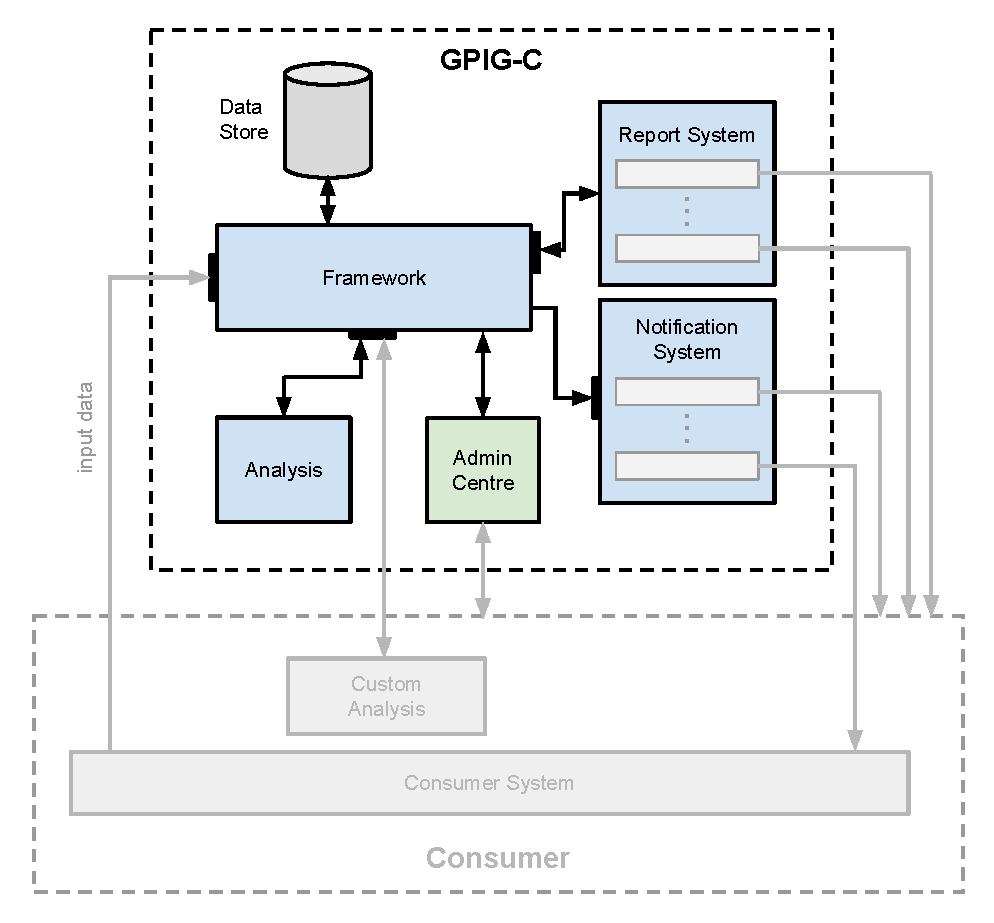
\includegraphics[width=0.75\textwidth]{system-architecture.pdf}
  \caption{System diagram}
\end{figure}

\section{Team organisation}

\subsection{Team members}

\subsection{Roles}


\section{Development plan}

\subsection{Software engineering methodology}

\subsection{Schedule}


\section{Risk register}


\section{Customer communication}


\end{document}
